\documentclass[a4paper, 12pt]{book}

% Basic Packages
\usepackage[utf8]{inputenc}
\usepackage{amsmath, amssymb, amsthm} % For math symbols and environments
\usepackage{graphicx} % For including images
\usepackage{hyperref}% For clickable links
\usepackage{xcolor} % For colors
\usepackage[Conny]{fncychap} % A style of presenting chapters
\usepackage[]{minted}
\usepackage{tcolorbox}
\usepackage{fancyvrb}
\usepackage[]{tikz}
\fvset{tabsize=4}

\usepackage[]{float}

% Configure minted settings
\setminted{
	breaklines=true,   % Automatically break long lines
	linenos=false,      % Show line numbers
	%frame=lines,       % Optional: Add a frame around the code
	fontsize=\footnotesize,  % Optional: Adjust font size
	tabsize=3,
	numbersep=10pt,
}


\graphicspath{{images/}{snippets/}}

\hypersetup{    % Here referencing is customized 
	colorlinks = true, % If true, the referencing texts will be colored
	linkcolor  = blue, % Texts referencing to some part of the same pdf will appear blue
	urlcolor   = red   % Texts linking to an URL will apper red
}

% Page layout
\usepackage{geometry}
\geometry{margin=1in}

% Custom Commands
\newcommand{\BigO}[1]{\mathcal{O}\left(#1\right)}
\newcommand{\code}[1]{\texttt{#1}}
\newcommand{\algo}[1]{\textbf{Algorithm: #1}}
\newcommand{\define}[1]{\textbf{Definition: #1}}

% Environments
\newtheorem{theorem}{Theorem}[section]
\newtheorem{definition}{Definition}[section]

% Header and Footer
\usepackage{fancyhdr}
\pagestyle{fancy}
\fancyhf{}
\fancyhead[L]{DSA Notes}
\fancyhead[R]{\thepage}

% Document Title
\title{Data Structures and Algorithms Notes}
\author{Soumik Seth}
\date{\today}

\begin{document}
	
	\maketitle
	\tableofcontents
	
	\chapter{C++ STL (Standard Template Libraries)}
	\section{Vectors}
	
		Vectors are sequence containers representing arrays that can change in size.	
		Just like arrays, vectors use contiguous storage locations for their elements, which means that their elements can also be accessed using offsets on regular pointers to its elements, and just as efficiently as in arrays. But unlike arrays, their size can change dynamically, with their storage being handled automatically by the container. Internally, vectors use a \underline{dynamically allocated array} to store their elements.
	
	\subsection{Declaring and initializing a vector} 
	\begin{itemize}
		\item \texttt{vector<int> v;} creates an empty container having size = 0
		\item \texttt{vector<int> v(5, 0);} creates a vector containing $five$ zeroes
		\item \texttt{vector<int> v\textsubscript{2}(v\textsubscript{1});} creates a vector containing all elements of v\textsubscript{1} in the \underline{same order}
		\item \texttt{vector<pair<int, int>> v;} creates a vector of pairs
			\begin{enumerate}
				\item \texttt{v = \{ \{1, 2\}, \{3, 4\}, \{5, 6\} \};}
				\item \texttt{v[0] == \{1, 2\}}
				\item \texttt{v[0].first == 1; v[0].second == 2;}
			\end{enumerate}
		\item \texttt{vector<tuple<int, int, int>> v;} creates a vector of tuples
			\begin{enumerate}
				\item \texttt{v = \{ \{1, 2, 3\}, \{4, 5, 6\} \};}
				\item \texttt{v[0] == \{1, 2, 3\}}
				\item \texttt{get<0>(v[0]) == 1}
				\item \texttt{get<1>(v[0]) == 2}
				\item \texttt{get<2>(v[0]) == 3}
			\end{enumerate}
		
	\end{itemize}
	\newpage
	
	\chapter{Data Structures}
	
	\section{Types of Data Structures}
	\begin{itemize}
		\item Linked Lists
		\item Stacks
		\item Queues
		\item Trees
		\item Graphs
	\end{itemize}
	
	\section{Linked Lists}
	A linked list is a linear data structure resembling a chain, where each node is connected to the next, and each node represents an individual element. Unlike arrays, the elements in a linked list are not stored in contiguous memory locations. Every node in a linked list contains two pieces of information, the \textbf{data} of node and \textbf{pointer} to the next node.
	\\ \\
	Unlike arrays, the size of linked lists can be increased or decreased easily.
	\\
	
	\begin{figure}[h]
		\centering
		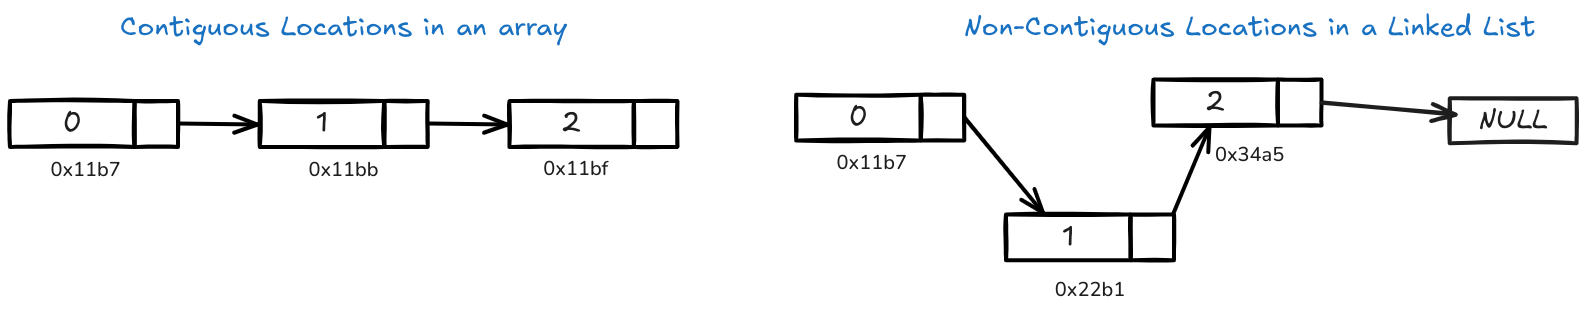
\includegraphics[width=1.1\textwidth]{LLarray.png}
		\caption{Array v/s Linked List}
		\label{fig:LLvarray}
	\end{figure}
	
	
	\subsection{Creating a linked list}
	\begin{figure}[H]
		\centering
		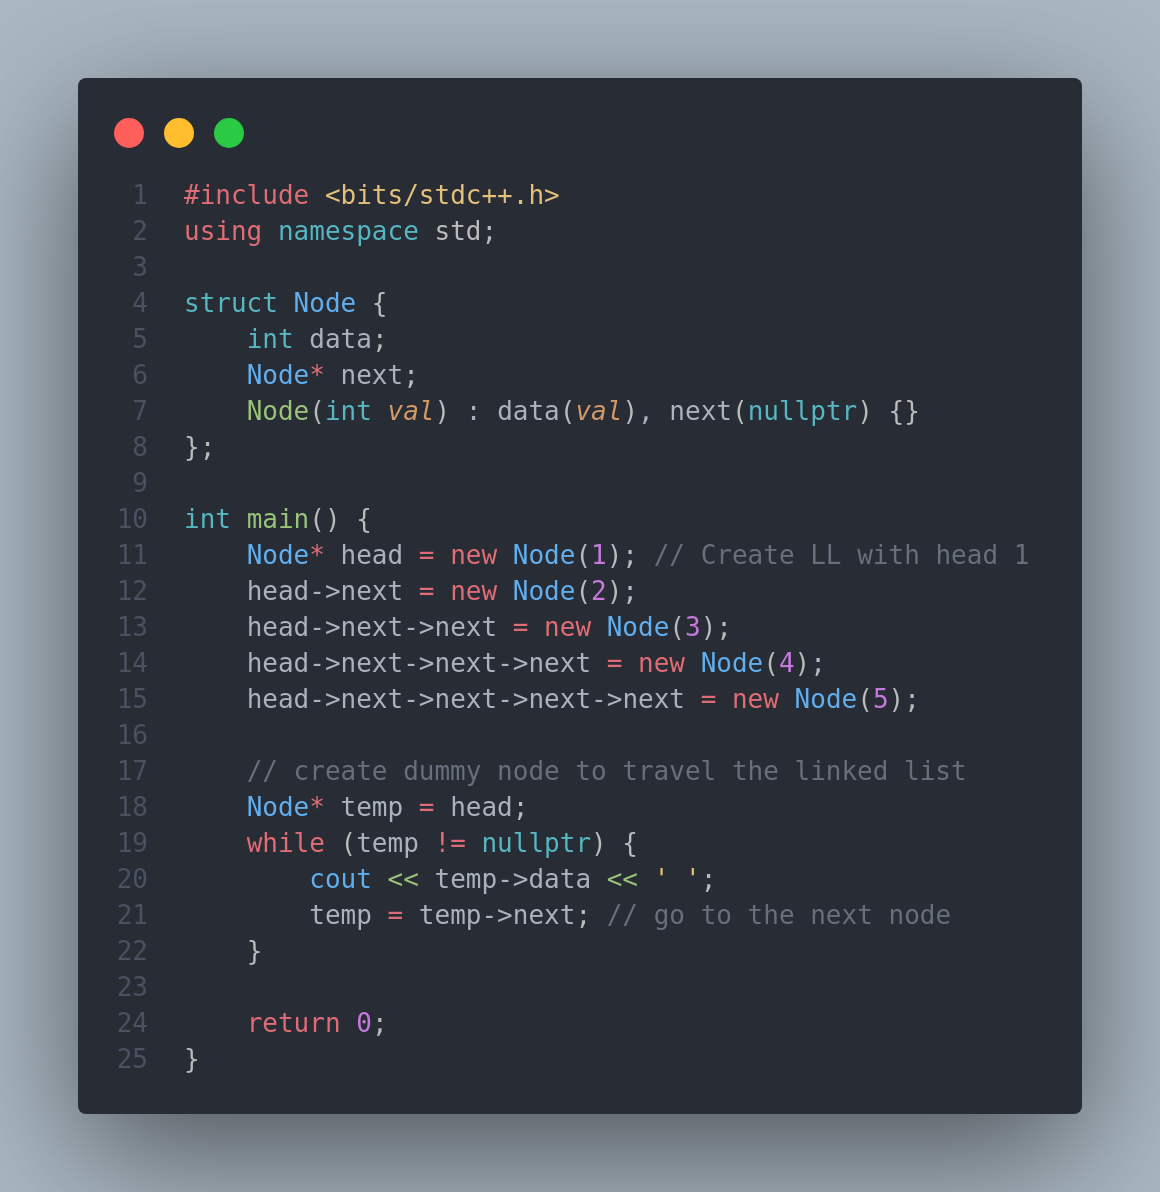
\includegraphics[width=\textwidth]{CreateLL.png}
		\label{fig:CreateLL}
	\end{figure}
	
	The above code produces a linked list that looks like this:
	
	\begin{figure}[h]
		\vspace{2mm}
		\centering
		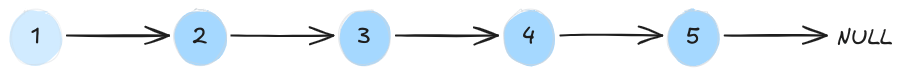
\includegraphics[width=0.8\textwidth]{1to5ll.png}
		\label{fig:1to5ll}
	\end{figure}
	
	\subsection{Types of linked lists}
	\subsubsection{Singly Linked Lists}
	In a singly linked list, each node points to the next node in the sequence. Traversal is straightforward but limited to moving in one direction, from the head to the tail.
	
	\subsubsection{Doubly Linked Lists}
	In this type, each node points to both the next node and the previous node, allowing for bidirectional connectivity.
	\begin{figure}[h]
		\vspace{-2mm}
		\centering
		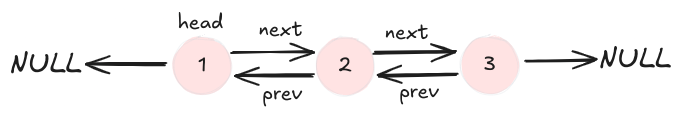
\includegraphics[width=0.7\textwidth]{1to3dll.png}
		\label{fig:1to3dll}
	\end{figure}
	
	\subsubsection{Circular Linked Lists}
	In a circular linked list, the last node points back to the head node, forming a closed loop.
	\begin{figure}[h]
		\vspace{-2mm}
		\centering
		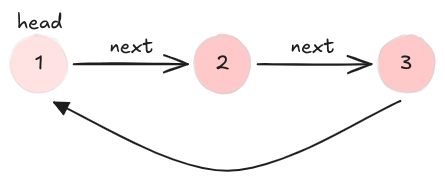
\includegraphics[width=0.5\textwidth]{1to3cll.png}
		\label{fig:1to3cll}
	\end{figure}
	
	\subsection{Creating a linked list from an array}
		\begin{figure}[h]
		\vspace{-2mm}
		\centering
		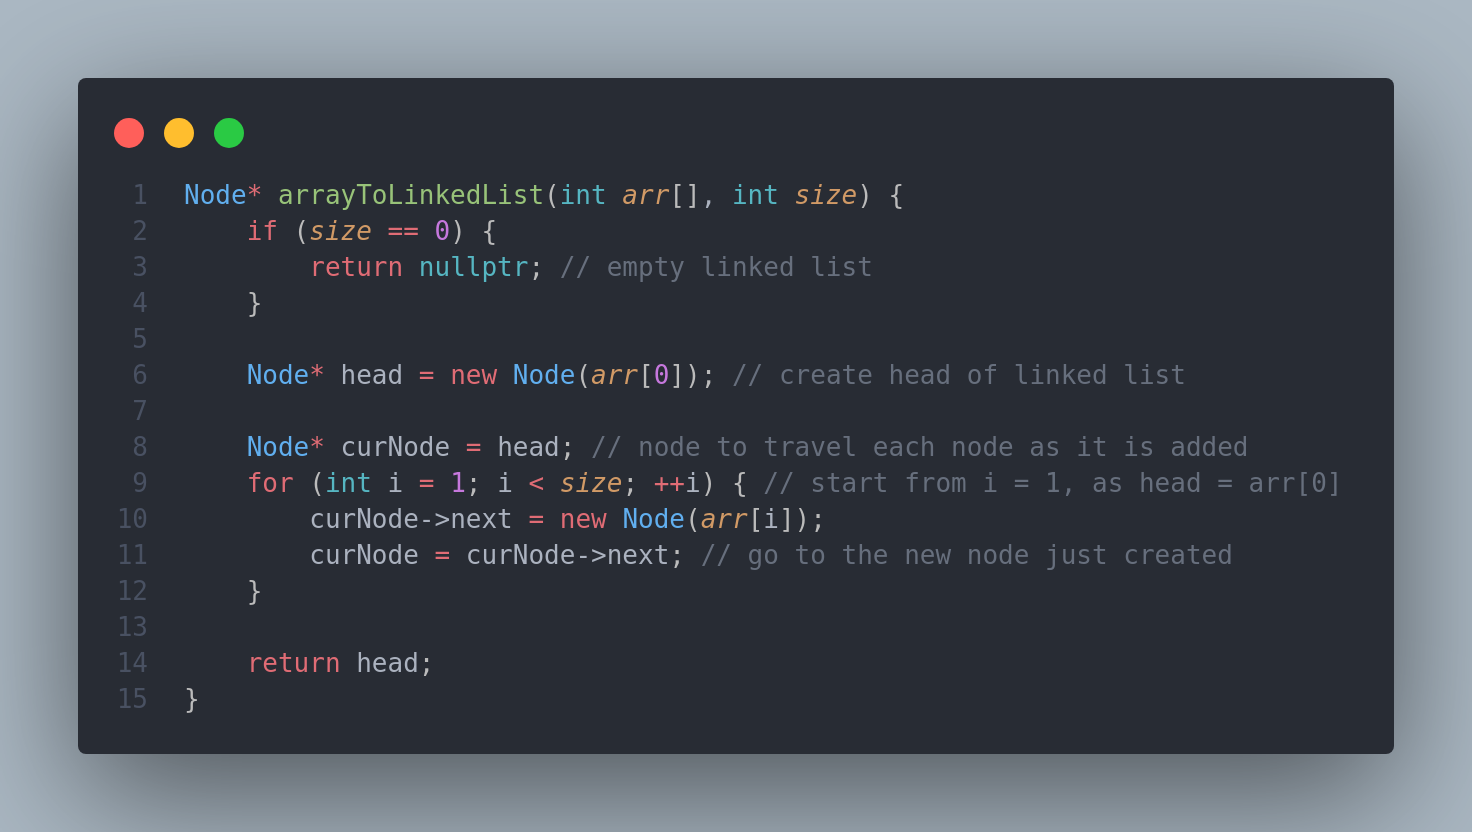
\includegraphics[width=\textwidth]{ArrToLL.png}
		\label{fig:ArrtoLL}
	\end{figure}
	\newpage
	\subsection{Find length of linked list}
	\begin{figure}[h]
		\vspace{-2mm}
		\centering
		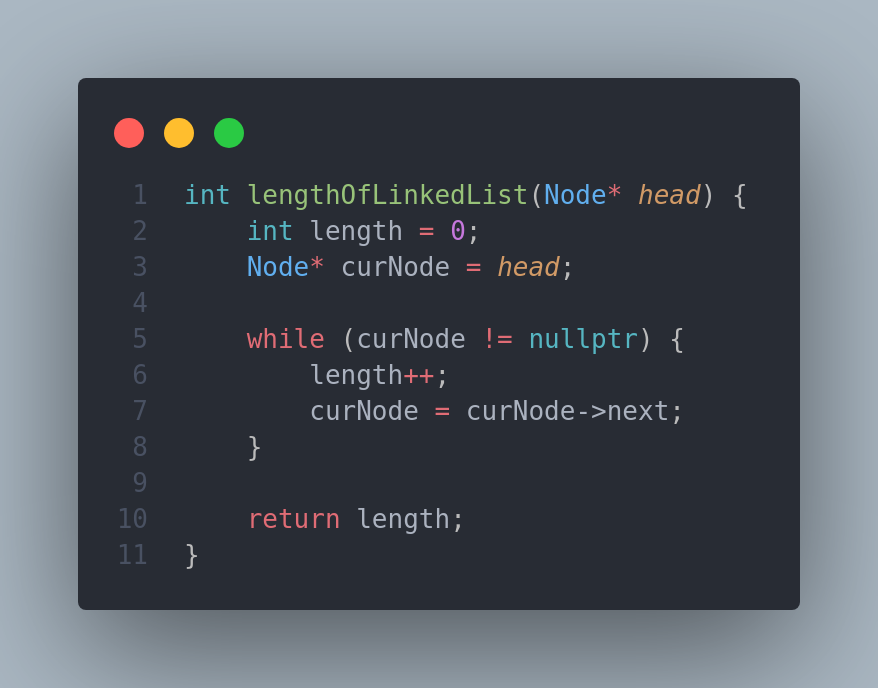
\includegraphics[width=0.8\textwidth]{LengthOfLL.png}
		\label{fig:LengthOfLL}
	\end{figure}
	
	\subsection{Delete head of linked list}
	\begin{figure}[h]
		%\vspace{3mm}
		\hspace{-7mm}
		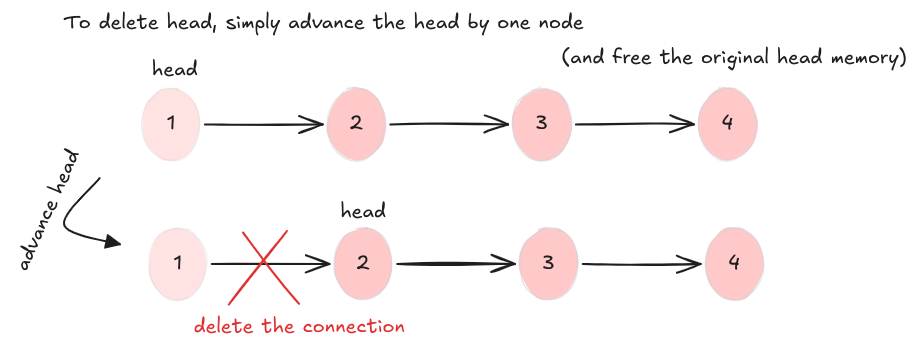
\includegraphics[width=1.1\textwidth]{deletehead.png}
		\caption{Delete head of a linked list}
		\label{fig:deletehead}
		
	\end{figure}
	
	\begin{figure}[H]
		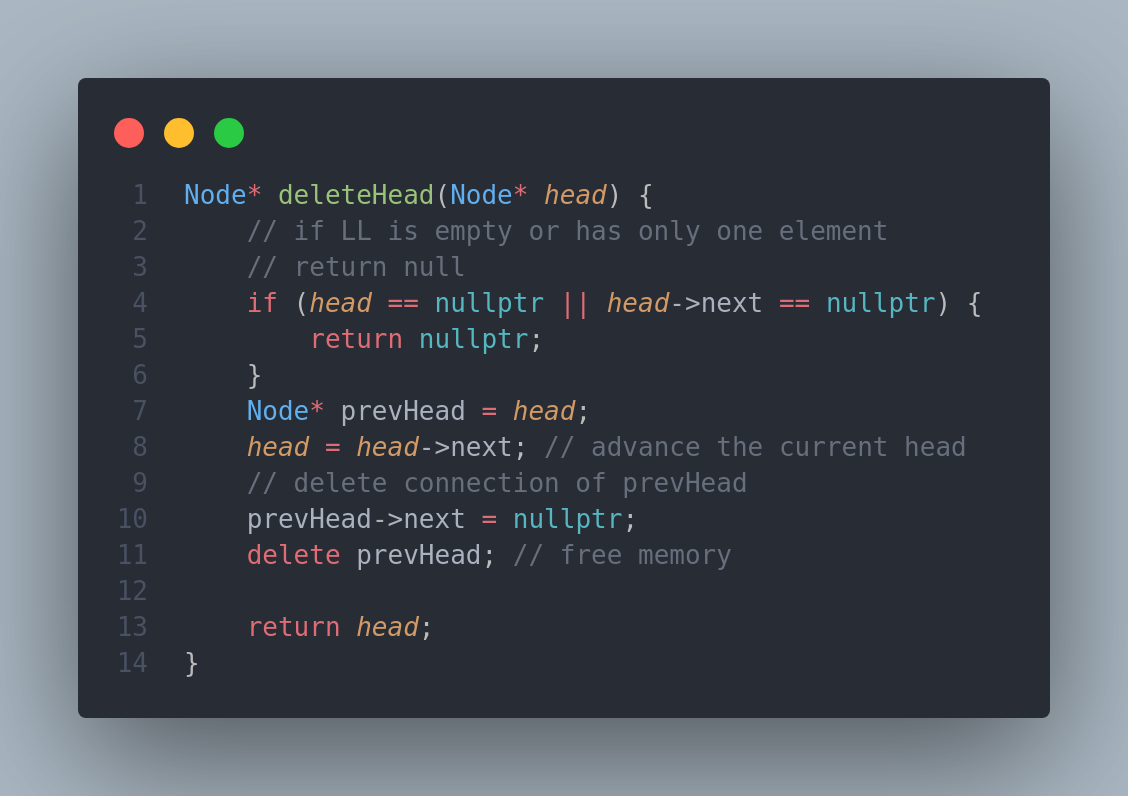
\includegraphics[width=\textwidth]{deleteheadcode.png}
		\label{fig:deleteheadcode}
	\end{figure}
	
	\subsection{Delete tail of a linked list}
	\begin{figure}[H]
		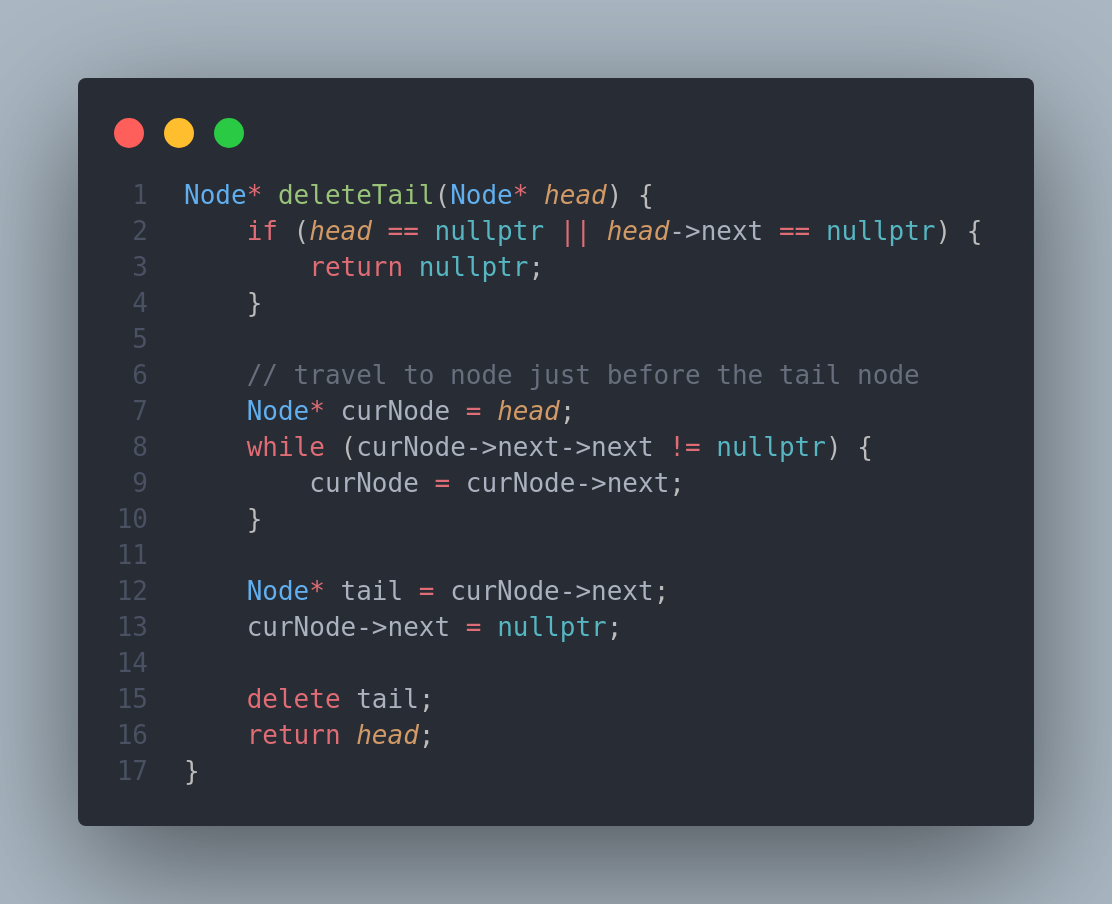
\includegraphics[width=0.8\textwidth]{deletetailcode.png}
		\label{fig:deletetailcode}
	\end{figure}
	
	\subsection{Delete K$^{th}$ element of a linked list}
	\begin{figure}[H]
		\hspace{-6mm}
		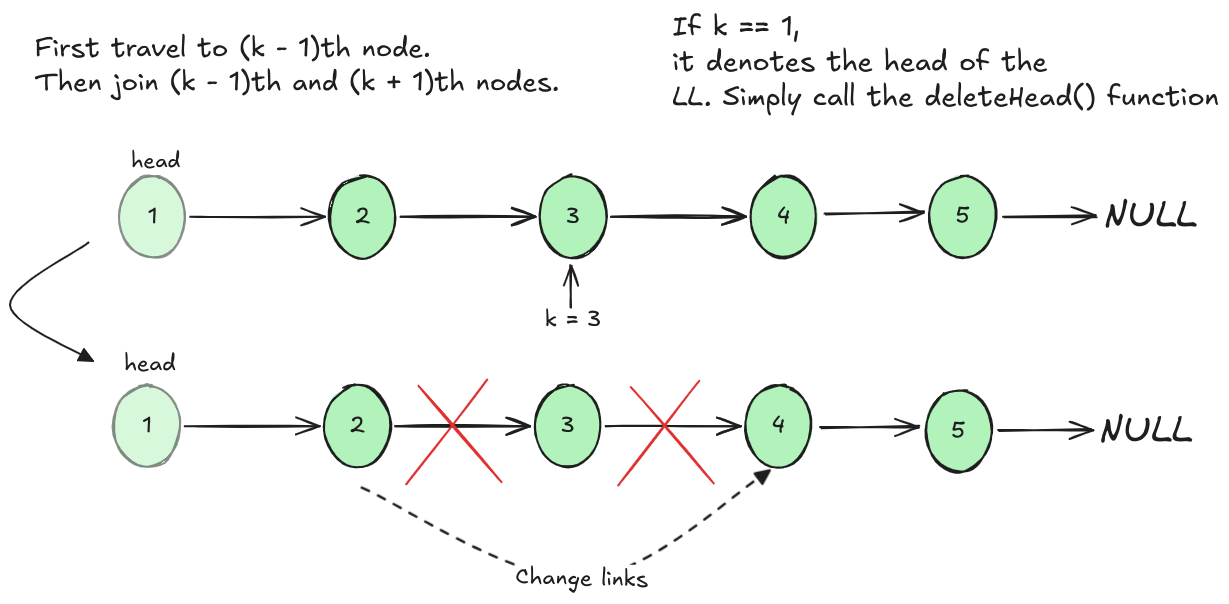
\includegraphics[width=1.1\textwidth]{deletekthnodecode.png}
		\label{fig:deletekthnodecode}
	\end{figure}
	\begin{figure}[H]
		\centering
		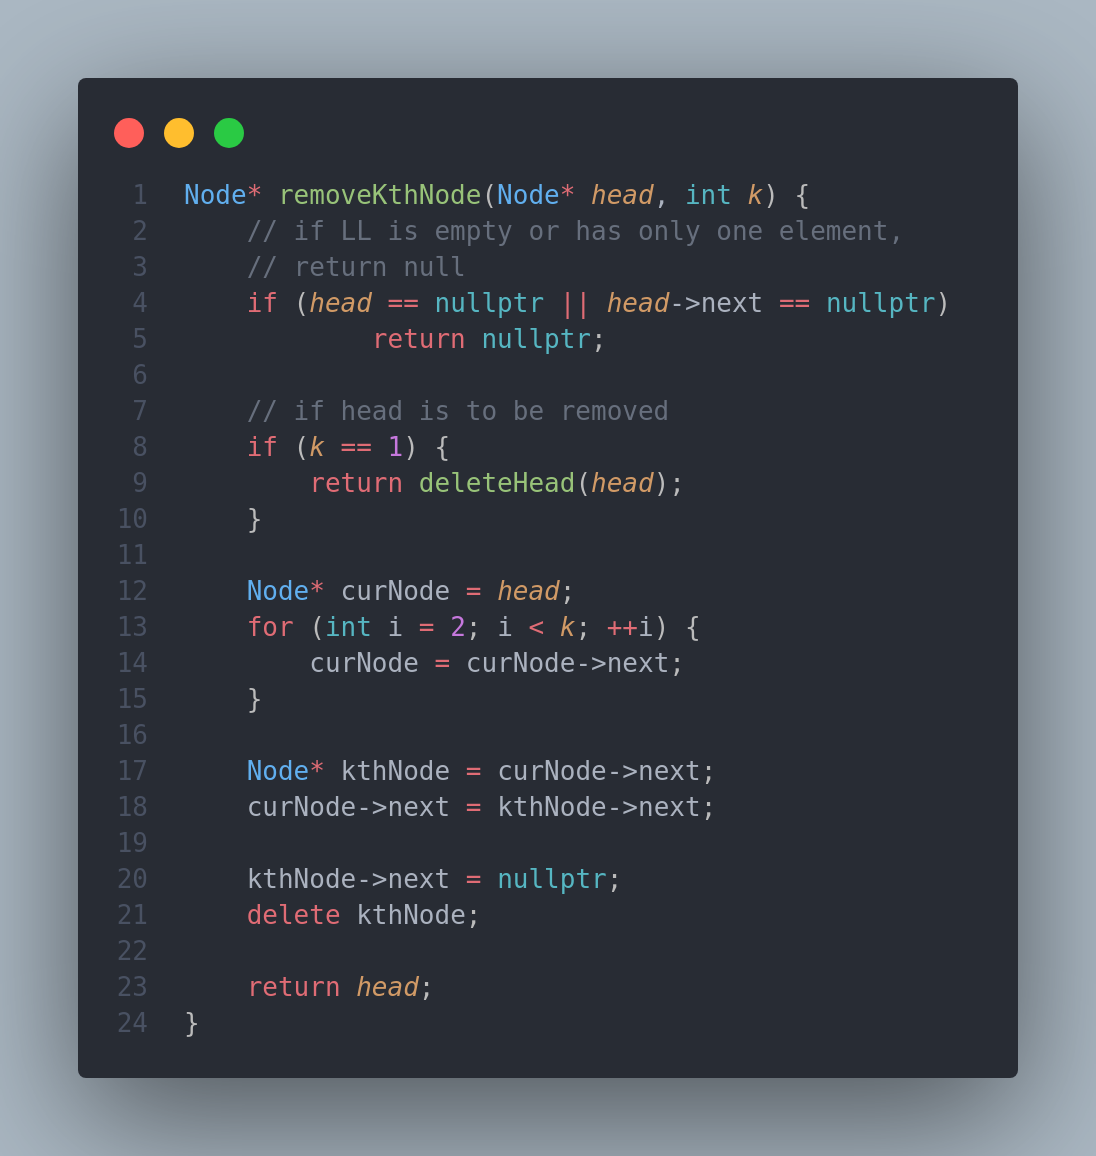
\includegraphics[width=0.8\textwidth]{deleteknode.png}
		\label{fig:deleteknode}
	\end{figure}
	\newpage
	
	\subsection{Find middle node of a Linked List}
		Here middle element refers to $\lfloor{\frac{n}{2}\rfloor}th$ element, where $n$ is the number of nodes in the linked list.
		The following approach can be used to do this efficiently- \\ \\
		Initialize 2 pointers, 
		\begin{itemize}
			\item \textbf{slow}: points to the head of linked list and travels node by node
			\item \textbf{fast}: points to the second node (if exists) and travels two nodes at a time
		\end{itemize}
		After this process is over, $i.e.$, when the fast pointer can no longer traverse the linked list, the slow pointer is pointing to the middle node of the linked list.
		
		\begin{figure}[h] 
			\centering
			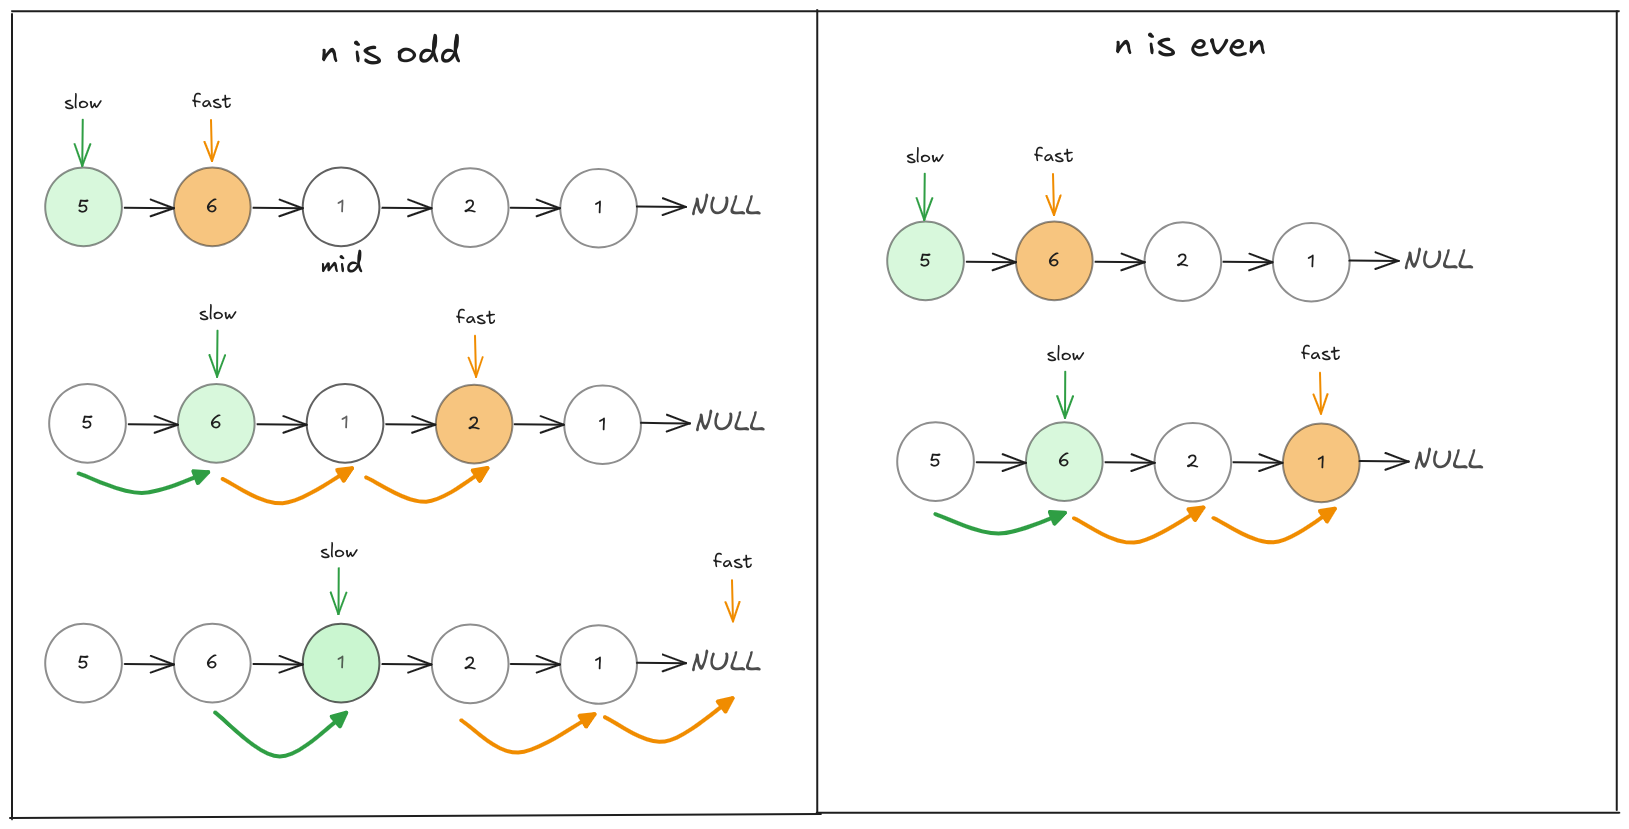
\includegraphics[width=1.1\textwidth]{midnode.png}
			\label{fig:findmidnode}
		\end{figure}
		
		
		\begin{tcolorbox}[]
			\begin{minted}[autogobble]{cpp}
Node* findMiddle(Node* head) {
	// if nodes <= 1, return immediately
	if (head == nullptr || head->next == nullptr) {
		return head;
	}
	Node* slow = head;
	Node* fast = head->next;
					
	while (fast != nullptr && fast->next != nullptr) {
		fast = fast->next->next;
		slow = slow->next; 
	}
					
	return slow;
}
			\end{minted}
		\end{tcolorbox}
		
	\newpage
	\section{Stacks}
	A stack is a linear data structure that follows the Last In, First Out (LIFO) principle. This means that the last element added to the stack will be the first one to be removed.
	\subsection{Implementing a stack using arrays} 
	
	\begin{itemize}
		\item push() : Pushes an element onto the stack
		\item pop() : Removes the topmost element from the stack \emph{and} returns it
		\item {top()} : Only returns the topmost element from the stack 
		\item {isEmpty()} : Returns $true$ if stack is empty else $false$
	\end{itemize}
	\vspace{\baselineskip}
	\subsection{Procedure}
	\begin{enumerate}
		\item 
	\end{enumerate}
	\newpage
	
	\begin{tcolorbox}[title=ArrayStack class]
		\begin{minted}{cpp}
			class ArrayStack {
			private:
				int topIndex;
				int maxSize;
				int* arr;
				
			public:
				ArrayStack(int size = 1000) {
					maxSize = size;
					arr = new int[maxSize];
					topIndex = -1; // denotes empty stack
				}
				
				// Destructor to free memory if object is not referenced anymore
				~ArrayStack() {
					delete[] arr;
				}
				
				void push(int x) {
					if (topIndex + 1 >= maxSize) {
						std::cout << "Stack overflow" << std::endl;
						return;
					}
					arr[++topIndex] = x;
				}
				
				int pop() {
					if (isEmpty()) {
						std::cout << "Stack is empty" << std::endl;
						return -1;
					}
					return arr[topIndex--];
				}
				
				int top() {
					if (isEmpty()) {
						std::cout << "Stack is empty" << std::endl;
						return -1;
					}
					return arr[topIndex];
				}
				
				bool isEmpty() {
					return topIndex == -1;
				}
			};
		\end{minted}
	\end{tcolorbox}
	
	\newpage
	
	\subsection{FAQs}
	\subsubsection{1. Next Greater Element}
	Given an array arr of size n containing elements, find the next greater element for each element in the array in the order of their appearance.
	The next greater element of an element in the array is the nearest element on the right that is greater than the current element.
	If there does not exist a next greater element for the current element, then the next greater element for that element is -1.
	\newline \\
	Example
		 Input:	
		
		
	
	\chapter{Sorting Algorithms}
	\section{Bubble Sort}
	
	\textbf{Description:} Repeatedly swaps adjacent elements if they are in the wrong order.
	\begin{tcolorbox}
	\begin{Verbatim}
void bubbleSort(int arr[], int n) {
	for (int i = 0; i < n - 1; i++) {
		for (int j = 0; j < n - i - 1; j++) {
			if (arr[j] > arr[j + 1])
				swap(arr[j], arr[j + 1]);
		}
	}
}
	\end{Verbatim}
\end{tcolorbox}
	
	\begin{itemize}
		\item \textbf{Time Complexity}: $\BigO{n^2}$
		\item \textbf{Space Complexity}: $\BigO{1}$
	\end{itemize}
	
	
	
	\section{Quick Sort}
	\textbf{Description:} A pivot is chosen which is then placed in its correct place (the pivot's position in the sorted array, called the \emph{partition index}). This step is then repeated for left and right portion of the pivot recursively.
	
	%\vspace{\baselineskip} 
	
	\begin{enumerate}
		\item \textbf{\underline{Recursion}}: Involves recursively calling the helper function
	
	\begin{tcolorbox}
	\begin{Verbatim}
void quickSortHelper(int arr[], int low, int high) {
	if (low < high) {
		int pIndex = partition(arr, low, high);
		quickSortHelper(arr, low, pIndex - 1);
		quickSortHelper(arr, pIndex + 1, high);
	}
}
	\end{Verbatim}
	\end{tcolorbox}
	
	\vspace{\baselineskip} 
	
	\item \textbf{\underline{Partition}}: Function that partitions the array and places the pivot in its correct place
	\begin{tcolorbox}
		\begin{Verbatim}
int partition(int arr[], int low, int high) {
	int pivot = arr[high];
	int i = low - 1;
	for (int j = low; j < high; ++j) {
		if (arr[j] <= pivot) {
			swap(arr[i + 1], arr[j]);
			i = i + 1;
		}
	}
	swap(arr[i + 1], arr[high]);
	return (i + 1);
}
		\end{Verbatim}
	\end{tcolorbox}
	\vspace{\baselineskip} 
\end{enumerate}


\begin{itemize}
	\item \textbf{Time Complexity}:
	\begin{itemize}
	
		\item Best Case = $\BigO{n \log n}$ 
		
		\item Average Case = $\BigO{n \log n}$ 
		
		\item Worst Case = $\BigO{n^2}$
	\end{itemize}
		
	\item \textbf{Space Complexity}: $\BigO{1}$ 
\end{itemize}
	
\end{document}
